\documentclass[12pt]{article}
\usepackage{amsmath}
\usepackage{graphicx}
\usepackage{hyperref}
\usepackage[latin1]{inputenc}
\usepackage{float}
\usepackage[a4paper, portrait, margin=0.5in]{geometry}

\graphicspath{ {./img/} }

\title{CS547 Assignment 2\\Test Case Prioritisation}
\author{Wojciech Cichoradzki\\201506554}
\date{23/10/2019}

\begin{document}
\maketitle

\section{Overview}
A Python 3 script was implemented which goal is to find the optimal solution for the Test Case Prioritisation problem using three different algorthmic approaches:
\begin{itemize}
  \item Random solution generation
  \item Hill climbing solution finding
  \item Genetic algorthm approach
\end{itemize}
In this paper I am going to show the evaluation of the results and how implementation was done.

\section{Implementation}
\subsection{Introduction}
Each test data consisted of comma-separated values consisting of a test id and 0-1 values indicating whether the singular fault was found by the test of not. A possible solution to the problem consists of a test suite i.e. a set of a number of tests. A test suite in my case was represented by the Individual class. Most important field is the genes field that contained an array of tests along other fields and methods.\\
To modify behaviour of the script, the config file is provided either via an optional command line flag argument (default is \texttt{config.json} file in the root the project. It specifies the test data file, type of algorithm as well as different settings for each algorithm. Each algorithm is time-limited. When the time limit is reached, the program prints the most optimal solution found in the given time alongside three different graphs - Fitness of the solution over generation/iteration, total APFD (average percent faults detected) of the individal and local APFD until the plateau is reached (no more faults were detected).
\subsection{Fitness function}
Fitness function consists of four weighted parameters:
\begin{enumerate}
  \item Completeness - fraction of faults detected in all tests
  \item Performance - how good is the choice of tests until all faults are detected (the less "repeating" tests i.e. tests that do not introduce any more faults detections the better)
  \item Total APFD - APFD of the entire test suite.
  \item Local APFD until plateau is reach i.e. further tests do not introduce more faults detections
\end{enumerate}
Each parameter and each parameter weight takes a float value between 0.0 to 1.0, hence the fitness value takes also a value between 0.0-1.0. Furthermore, theoretical highest fitness is 1.0, but in practice, with the finite set of available tests, it would be impossible due to the fact that the APFD would never reach 100\%.
Weights for each parameter were assigned using a heuristic observation of how algorithm performs. Completeness was set to be the highest priority for the test suite. After all, best test suites detect all the faults. After that the performance of the test suite was set to be second most important factor. The reason for that is that even if the test suite detects 100\% of the faults, but it requires 100 tests to reach it, while it can be reached in just 5 tests, it is not very well performing test suite. Ideally, tests suites should reach 100\% faults detected as soon as possible, with no initial tests not increasing the faults detection percentage ("repeating" steps). Performance was calculated using the following formula: (number\_of\_steps\_to\_plateau - repeating\_steps)/number\_of\_steps\_to\_plateau. Local and total APFD weights were assigned differently under different conditions. If the performance the solution was not set to highest value 1.0, total APFD would not matter at all, but the local APFD would be assigned a small weight. That's because if we didn't polished our performance i.e. test selection to reach ideally 100\% of fault detection, we should focus on that - make the performance as good as possible. Also, increasing total APFD is not that difficult, simply adding new tests after the maximum faults were detected, increses the length of the plateau, hence making the integral value larger, hence increasing total APFD. To conclude, the resulting weights for each parameter were:
\begin{enumerate}
  \item Completeness - 0.80
  \item Performance - 0.1
  \item Total APFD - 0 or 0.01 if performance is 1.0
  \item Local APFD - 0.1 or 0.09 if performance is 1.0
\end{enumerate}

\subsection{Settings}
My implementation of the genetic algorthm introduces aforementioned "individals" aka chromosomes that contains genes i.e. different tests.\\
The genetic operations supported by the algorithm are:
\begin{itemize}
  \item Single-point crossover
  \item Mutation
  \item Adding new random tests
  \item Removing random test
\end{itemize}
The selection of the parents is based on roulette wheel selection, that returns two unique parents. For both big and small datasets, same genetic algorithm parameters were used. They were chosen heuristically, by tweaking them back and forth until a steady increase in overall fitness was observed. The final configs are located in \textt{/configs} directory.
The best parameters I could find were:
\begin{itemize}
  \item Initial number of tests (genes) - 50
  \item Population size - 100
  \item Number of elites - 2
  \item Crossover, mutation, addition, removal chance - 0.2
\end{itemize}
For the small data set, time limit of 70 seconds was set and for the larger one - 8 minutes.
\subsection{Running the package}
In the root of the project run:\\
\texttt{python3 -m test\_case\_prioritazation.start -c <config\_file.json>}\\
For example:\\
\texttt{python3 -m test\_case\_prioritazation.start -c configs/ga\_small\_set.json}\\
Runs the genetic algorithm config using the small data set.

\section{Evaluation of results}

\subsection{Small dataset}

\begin{figure}[H]
  \centering
  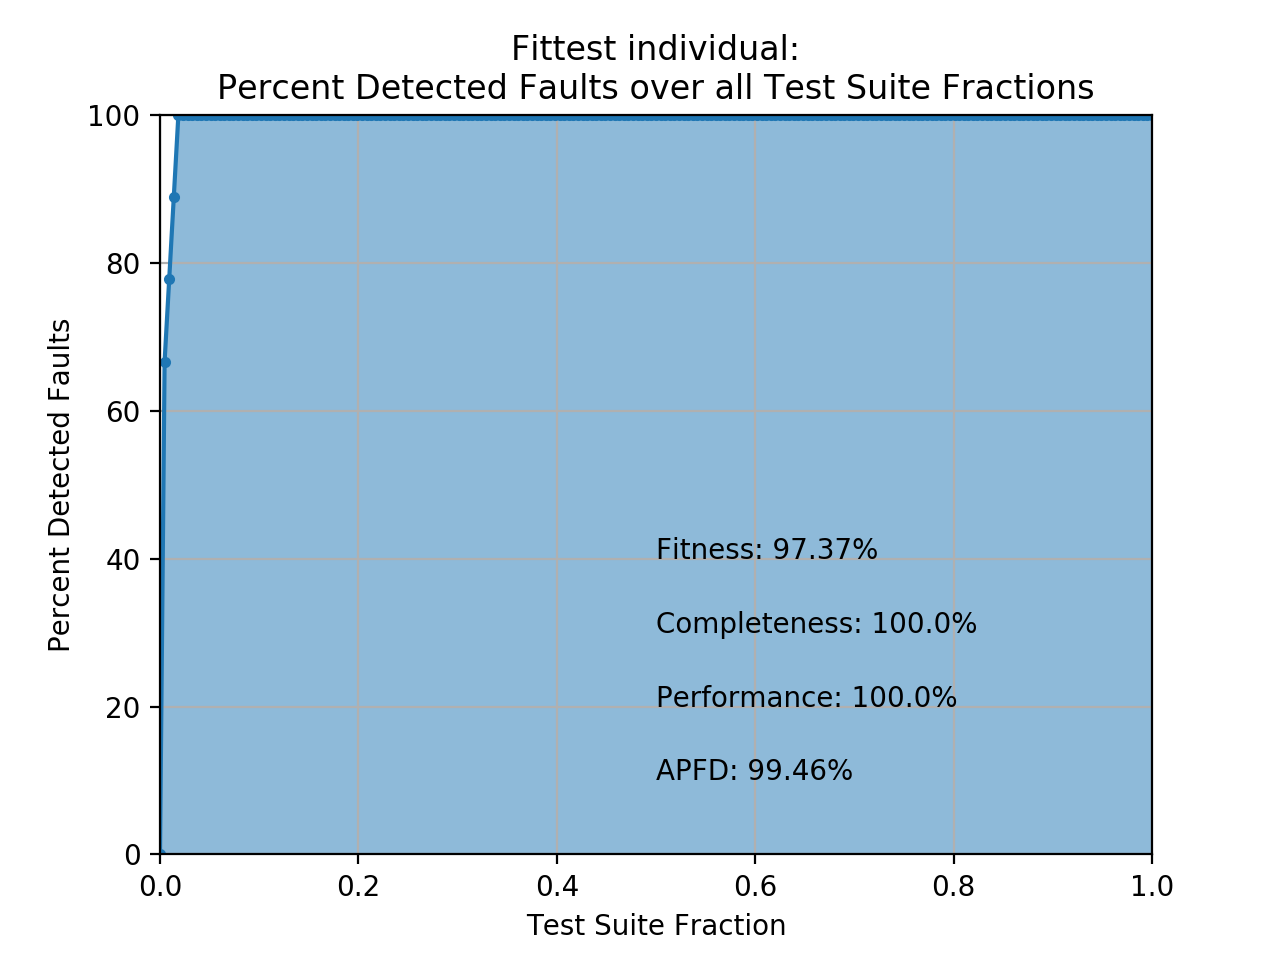
\includegraphics[width=0.49\textwidth]{ga_small_apfd_total}
  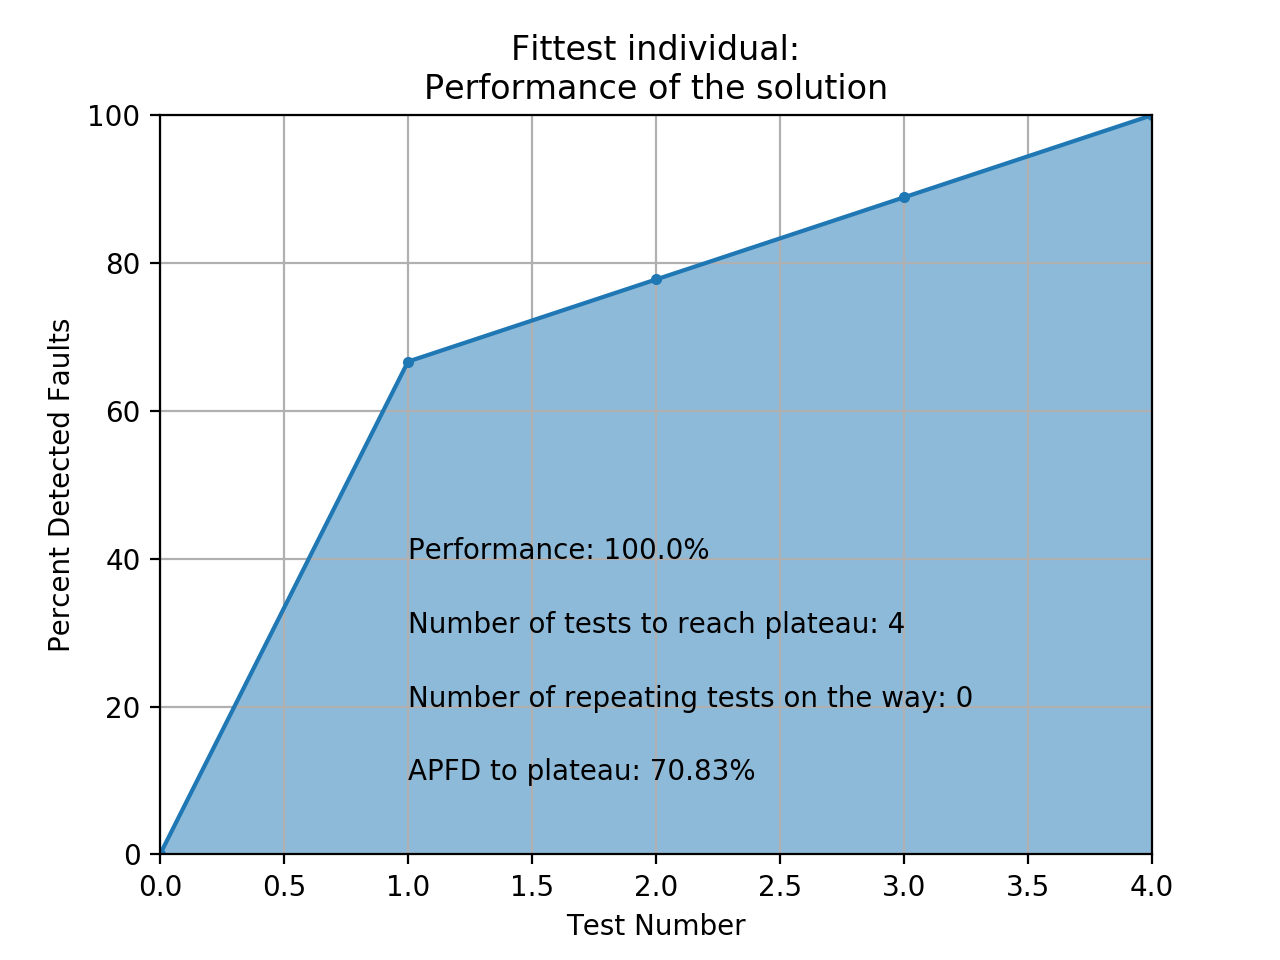
\includegraphics[width=0.49\textwidth]{ga_small_apfd_local}
  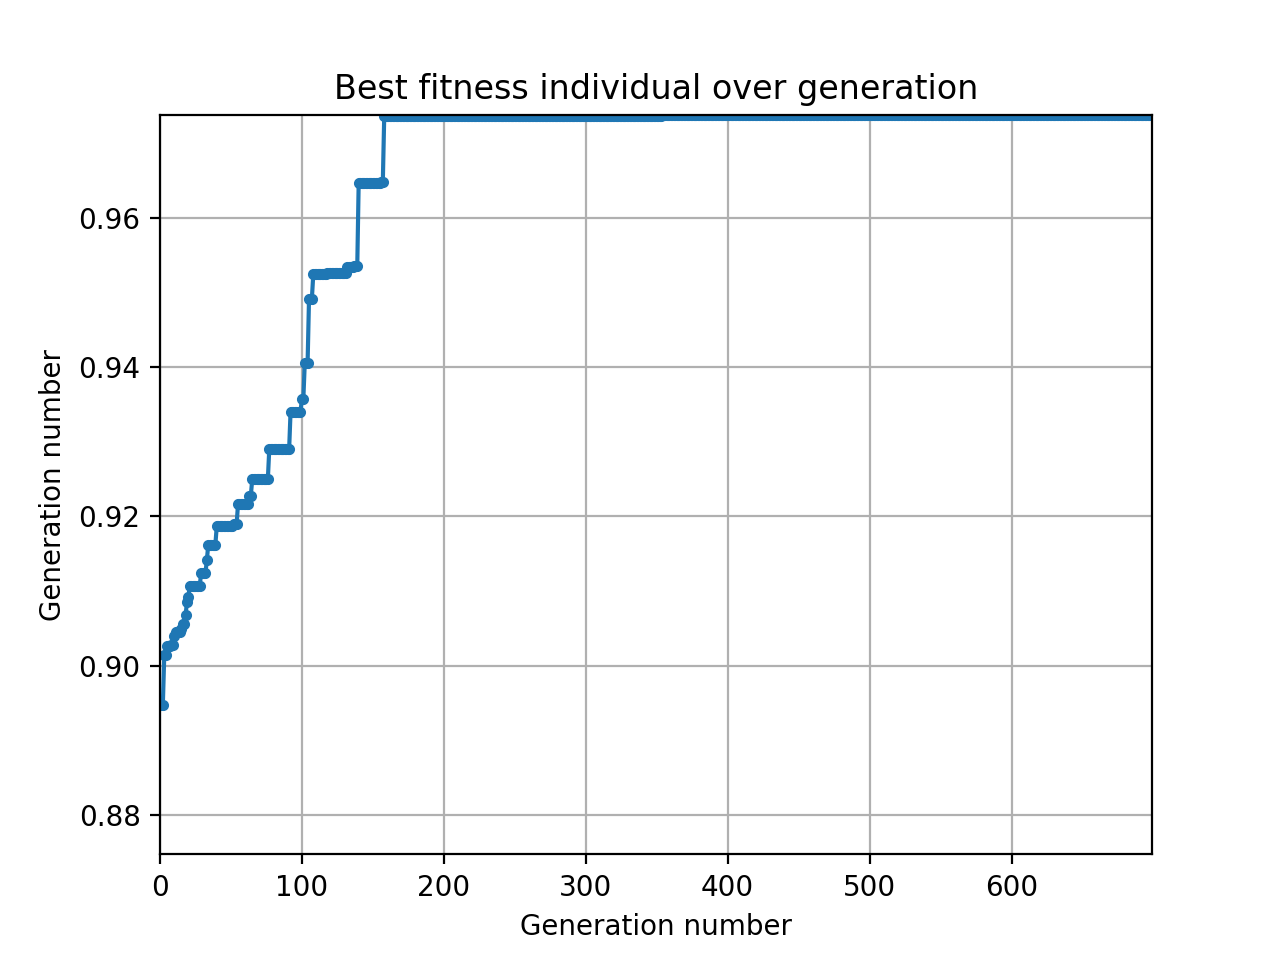
\includegraphics[width=0.6\textwidth]{ga_small_fitness_all}
  \caption{Statistics of running genetic algorithm over small data set}
  \label{fig:ga_small}
\end{figure}

\begin{figure}[H]
  \centering
  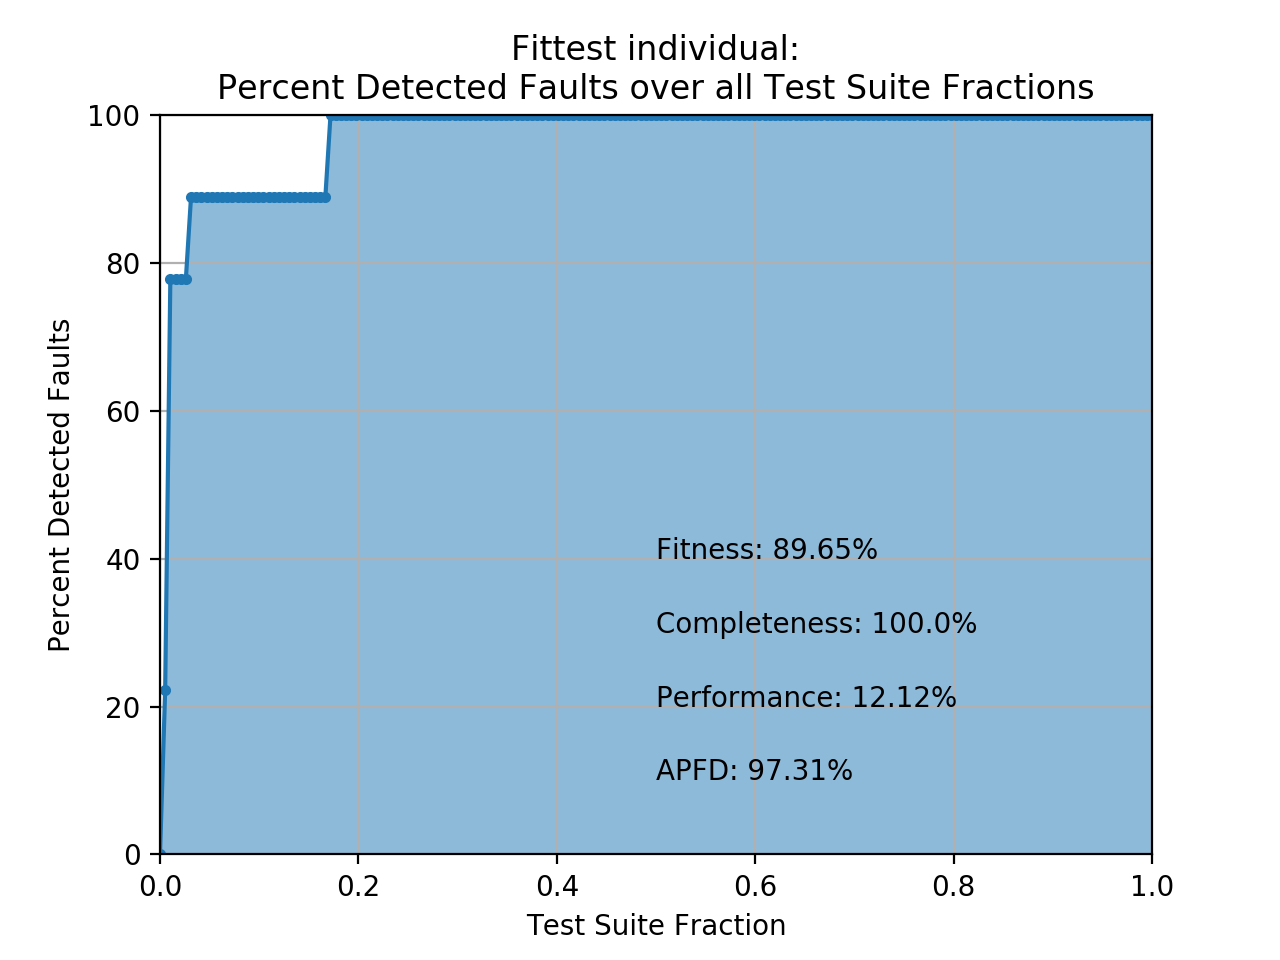
\includegraphics[width=0.49\textwidth]{hill_climber_small_apfd_total}
  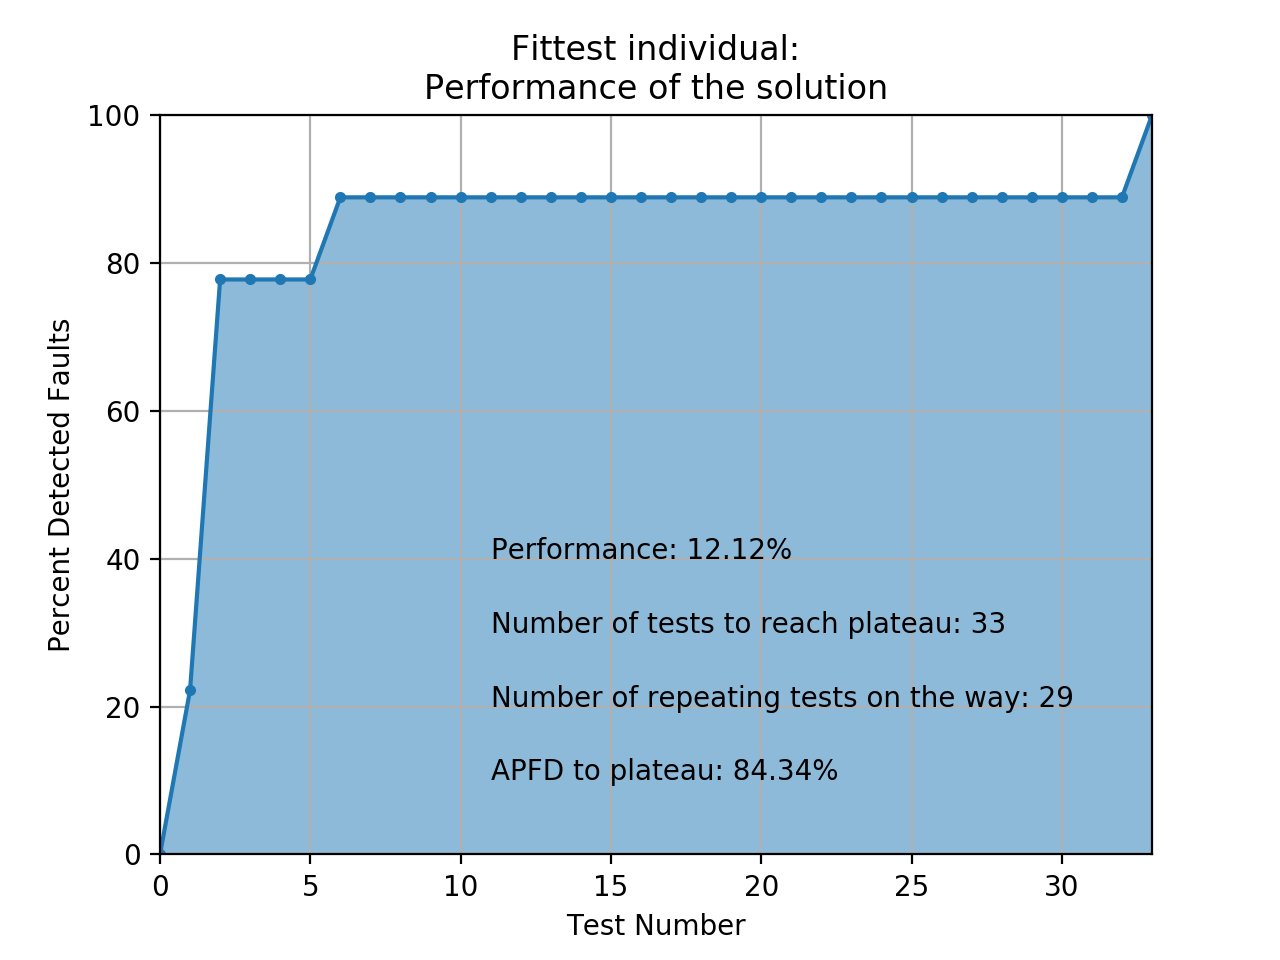
\includegraphics[width=0.49\textwidth]{hill_climber_small_apfd_local}
  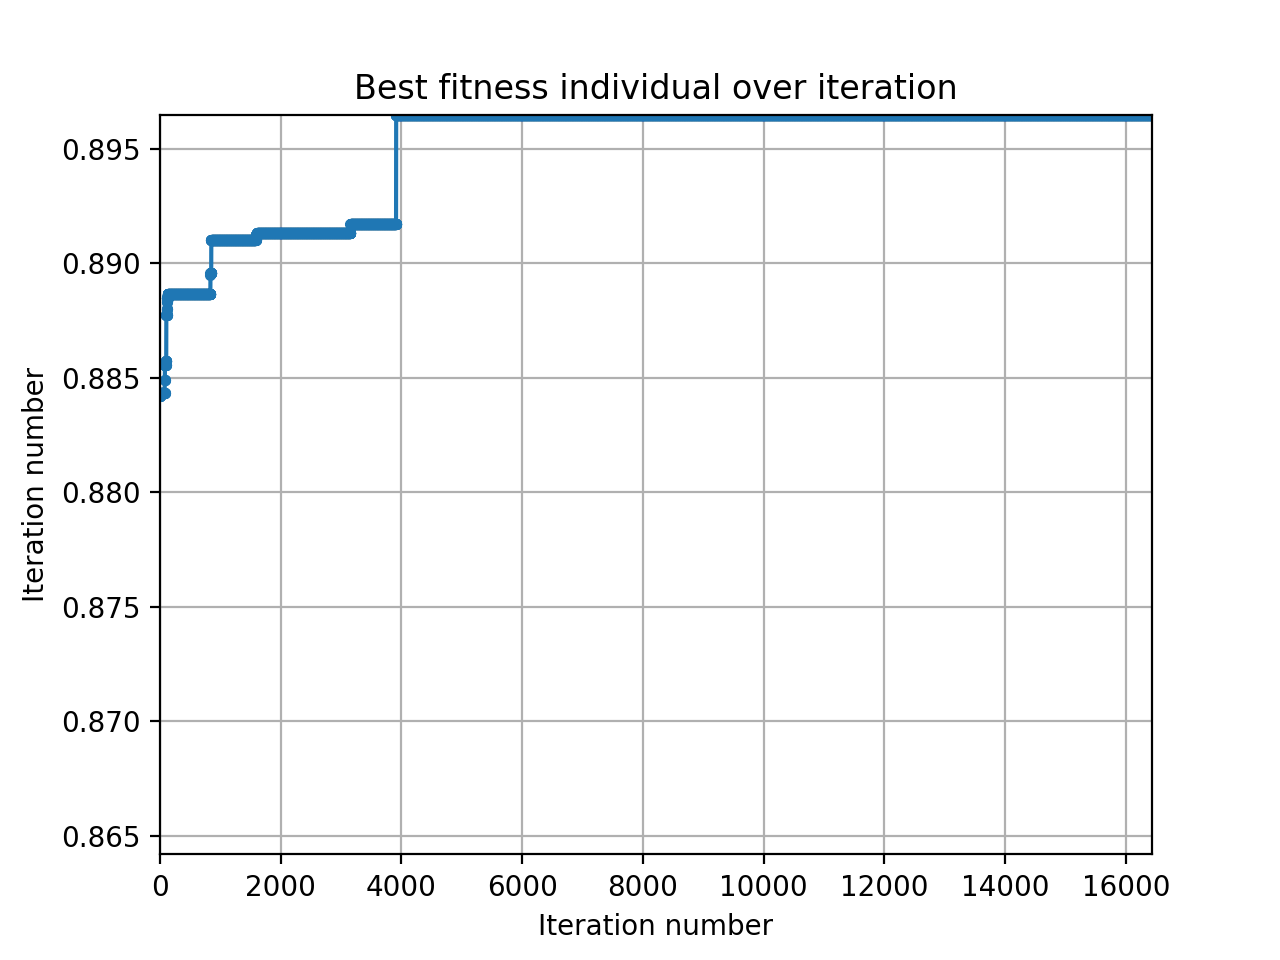
\includegraphics[width=0.6\textwidth]{hill_climber_small_fitness_all}
  \caption{Statistics of running hill climber algorithm over small data set}
  \label{fig:hill_climber_small}
\end{figure}

\begin{figure}[H]
  \centering
  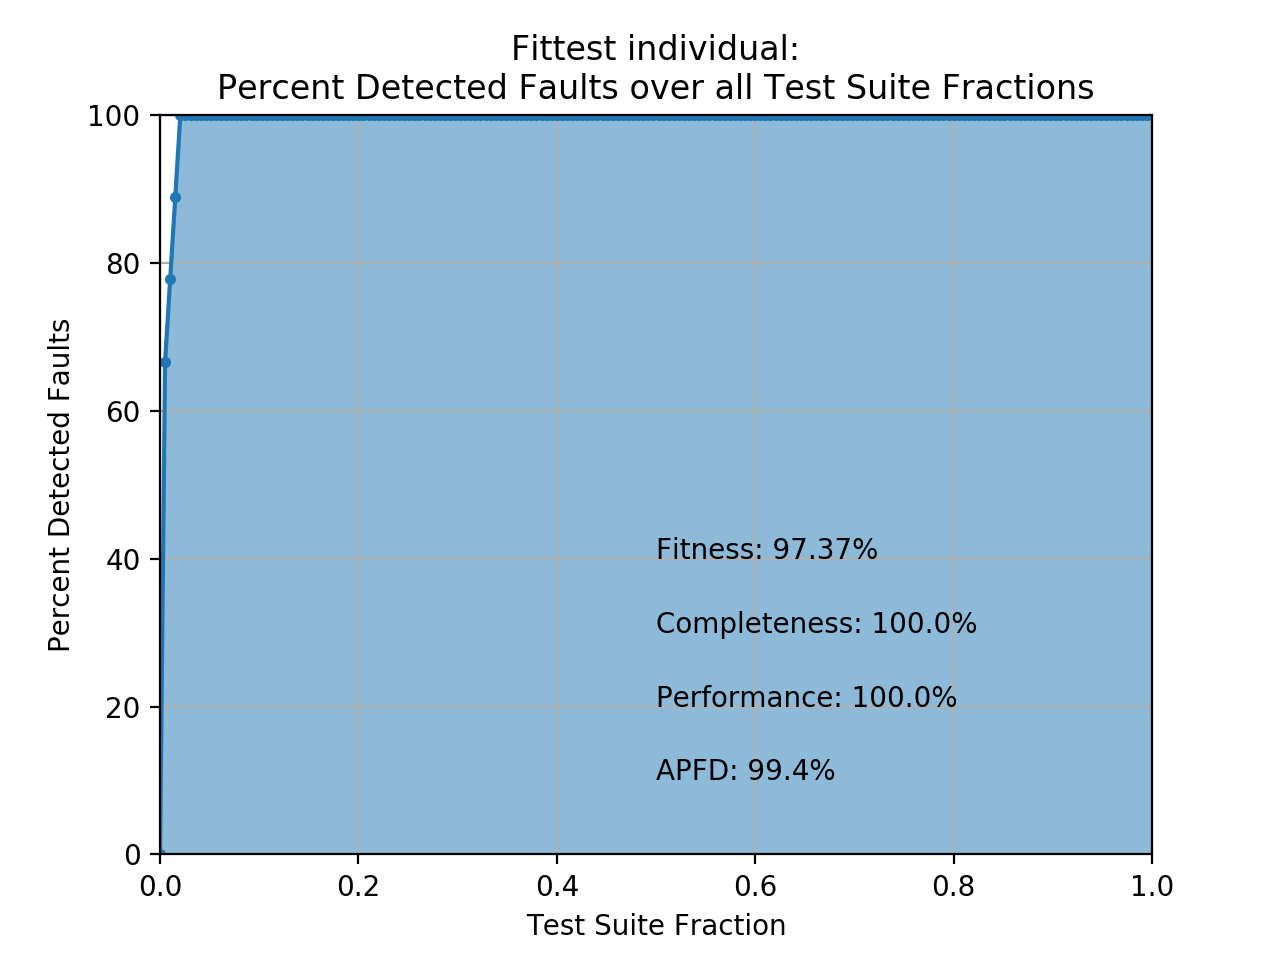
\includegraphics[width=0.49\textwidth]{random_small_apfd_total}
  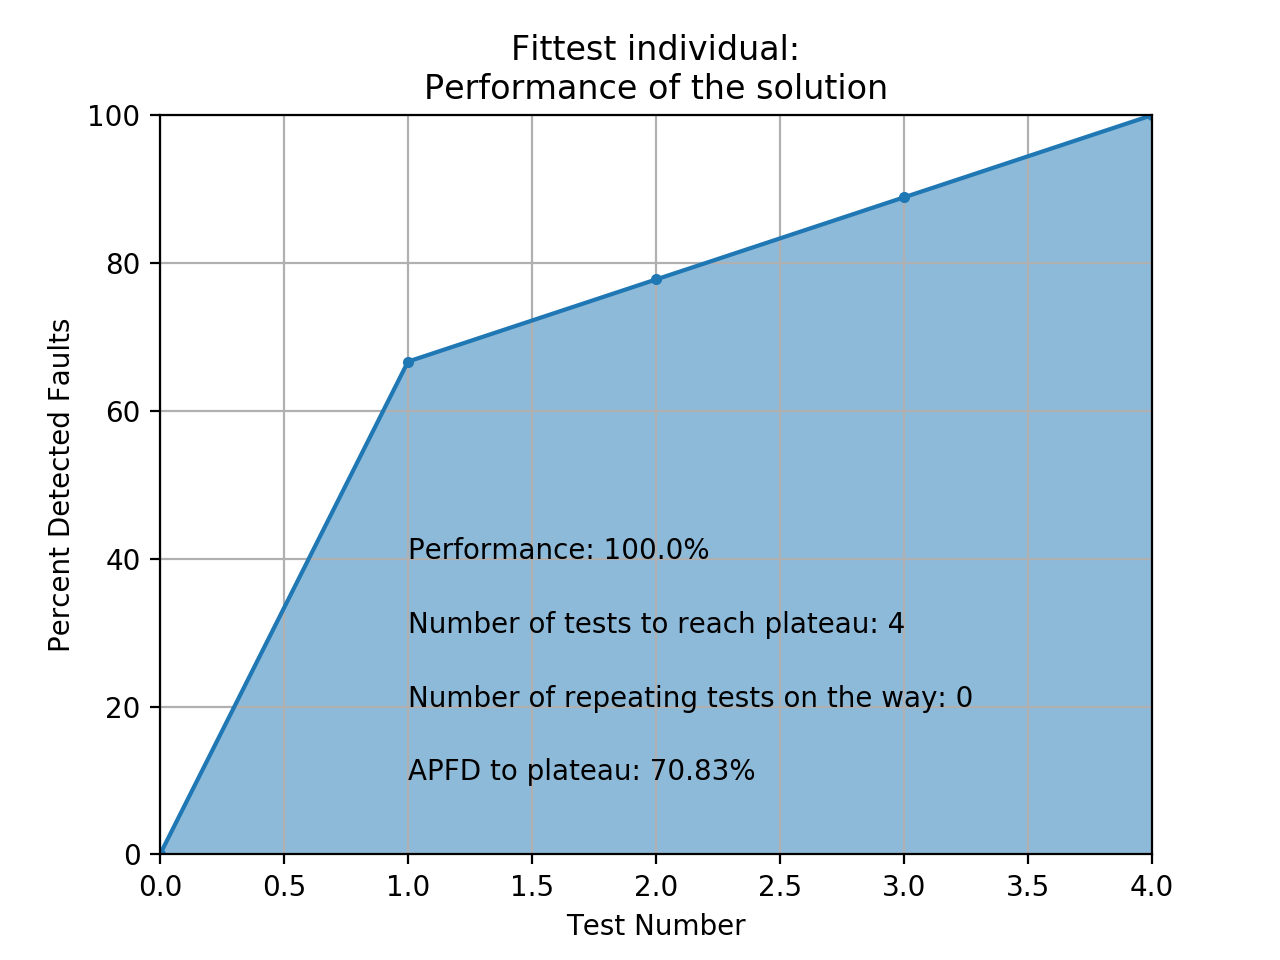
\includegraphics[width=0.49\textwidth]{random_small_apfd_local}
  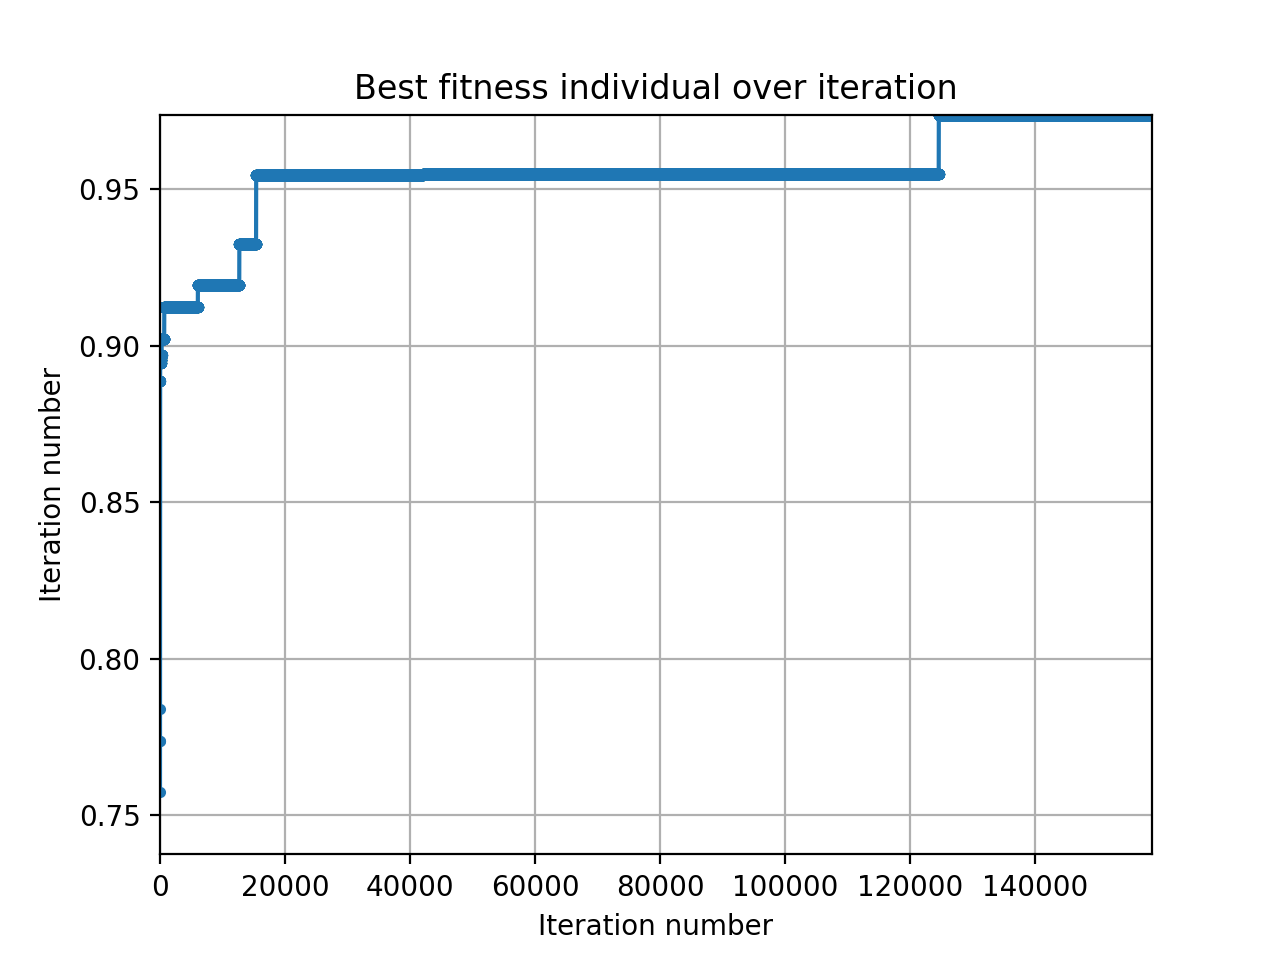
\includegraphics[width=0.6\textwidth]{random_small_fitness_all}
  \caption{Statistics of running random algorithm over small data set}
  \label{fig:random_small}
\end{figure}

Comparing figures \ref{fig:ga_small}, \ref{fig:hill_climber_small} and \ref{fig:random_small} it can observed that all algorithms provided solution that find 100\% of faults (Completeness) compared to 100\% in GA and Random. However, when it comes to other parameters, genetic algorithm and random solution outperformed hill climber, scoring 100\% in Performance and providing the optimal Local APFD at 70.83\%. Genetic algorthm had a slight advantage over the random solution by generating higher total APFD by 0.06 percentage points. Hill climber, even though it provided a complete solution, it takes 33 steps to reach 100\% detected faults comparing to only 4 generated by GA and Random algorithms. This yields to a better local APFD of the Hill Climber - 84.34\%, but at the cost of much worse performance at only 12.12\%.

\subsection{Big dataset}

\begin{figure}[H]
  \centering
  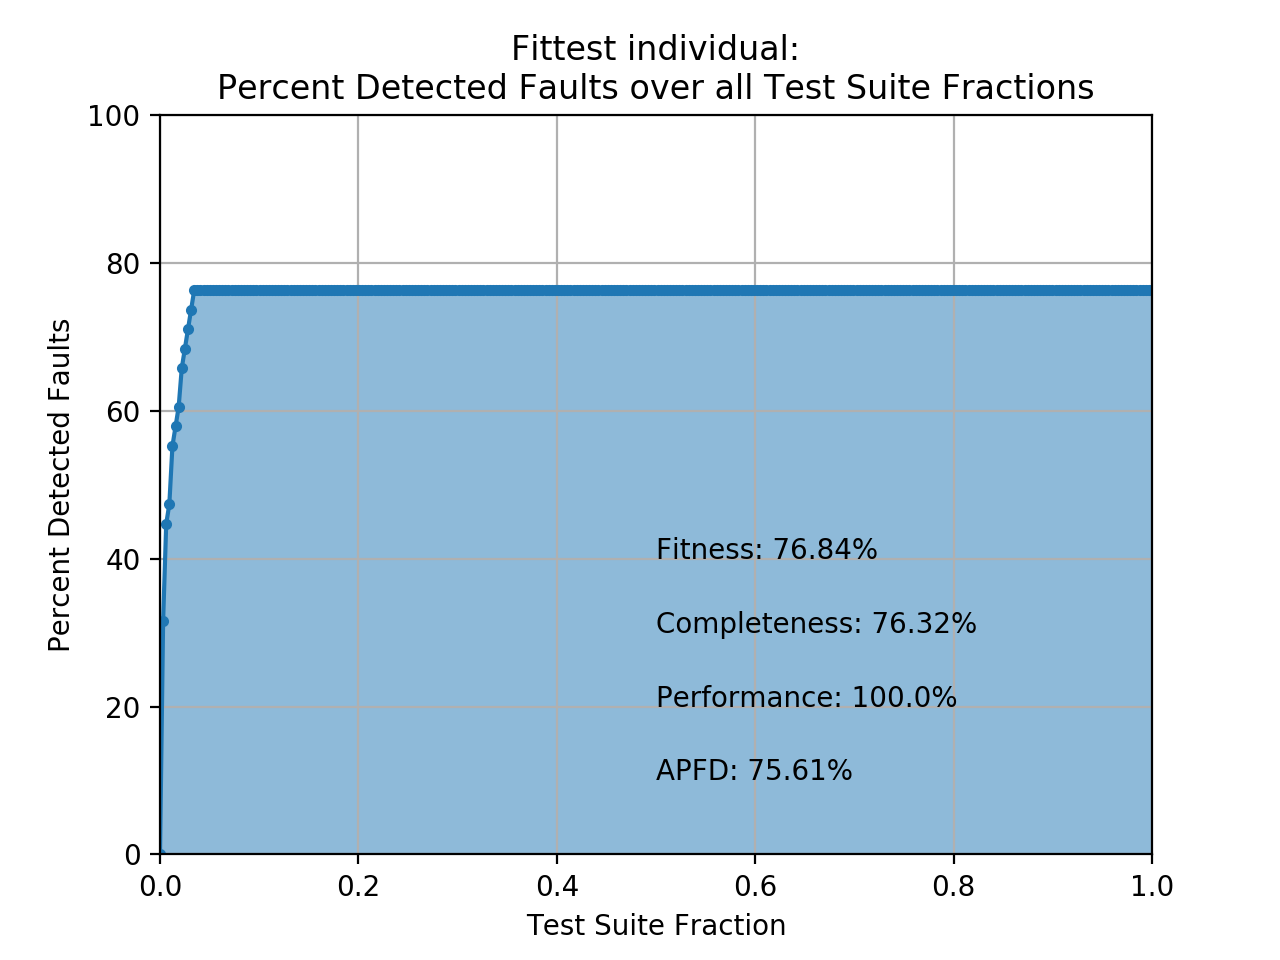
\includegraphics[width=0.49\textwidth]{ga_big_apfd_total}
  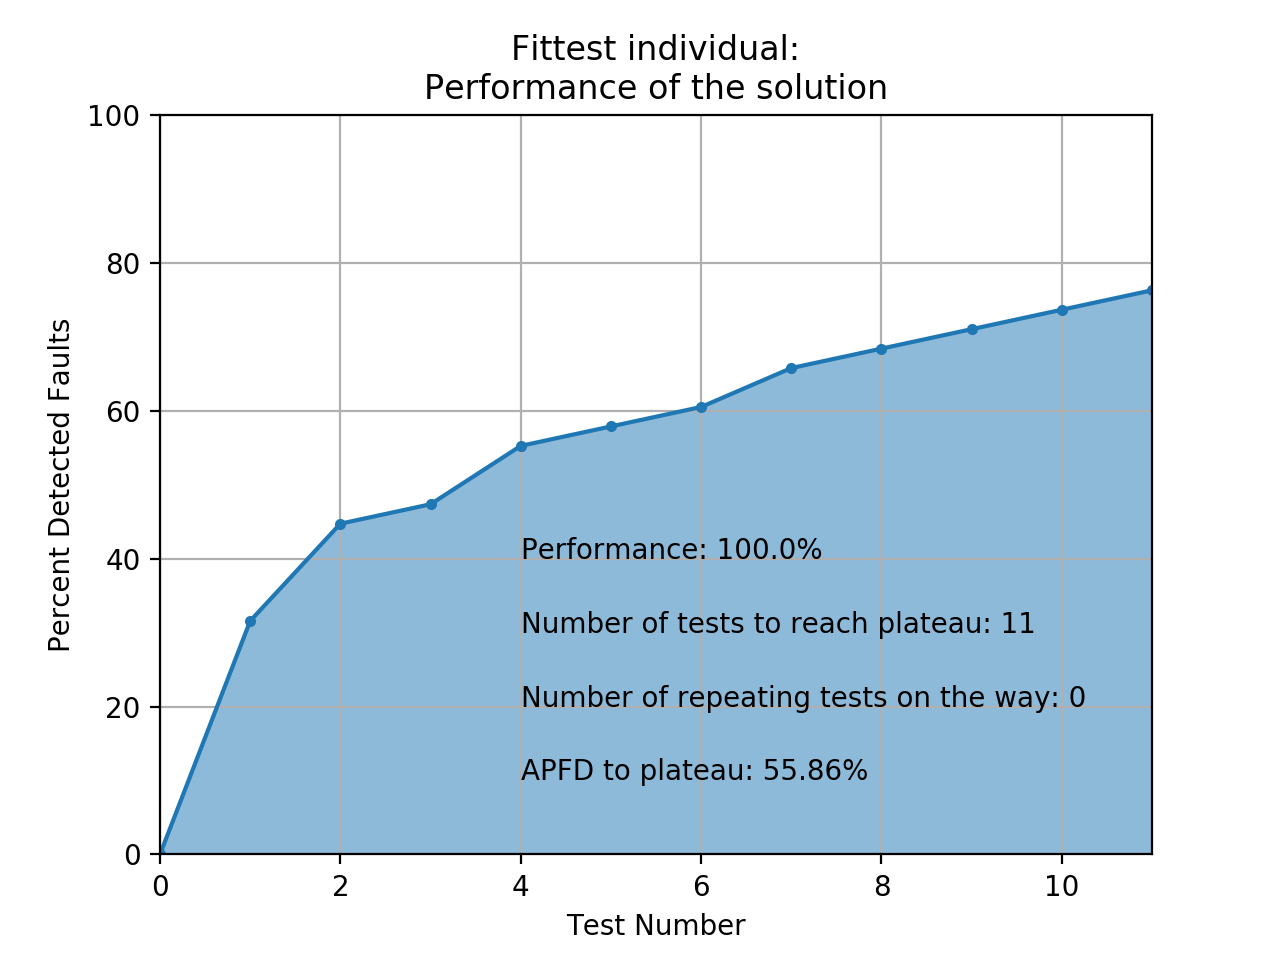
\includegraphics[width=0.49\textwidth]{ga_big_apfd_local}
  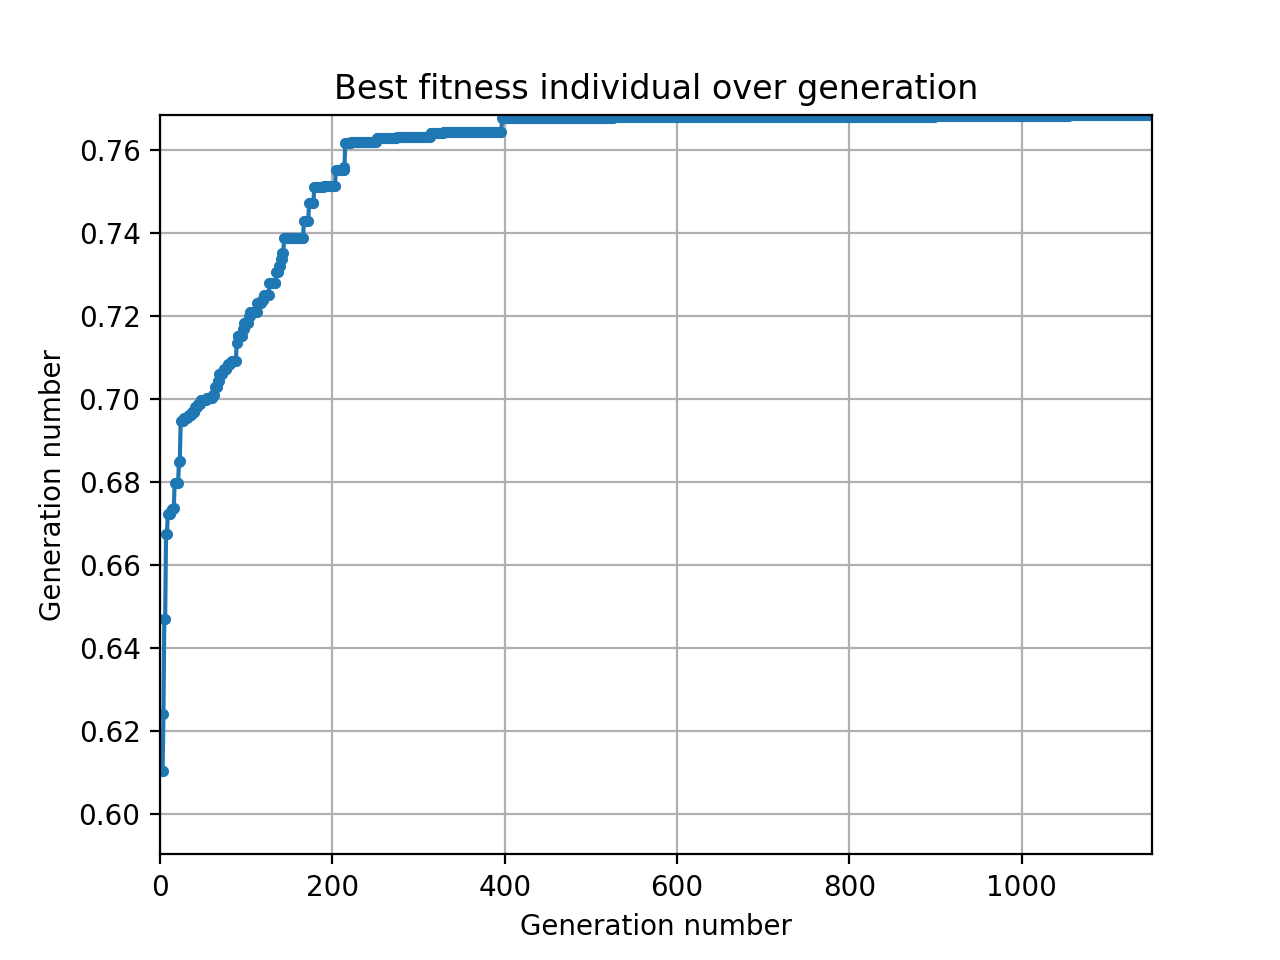
\includegraphics[width=0.6\textwidth]{ga_big_fitness_all}
  \caption{Statistics of running genetic algorithm over big data set}
  \label{fig:ga_big}
\end{figure}

\begin{figure}[H]
  \centering
  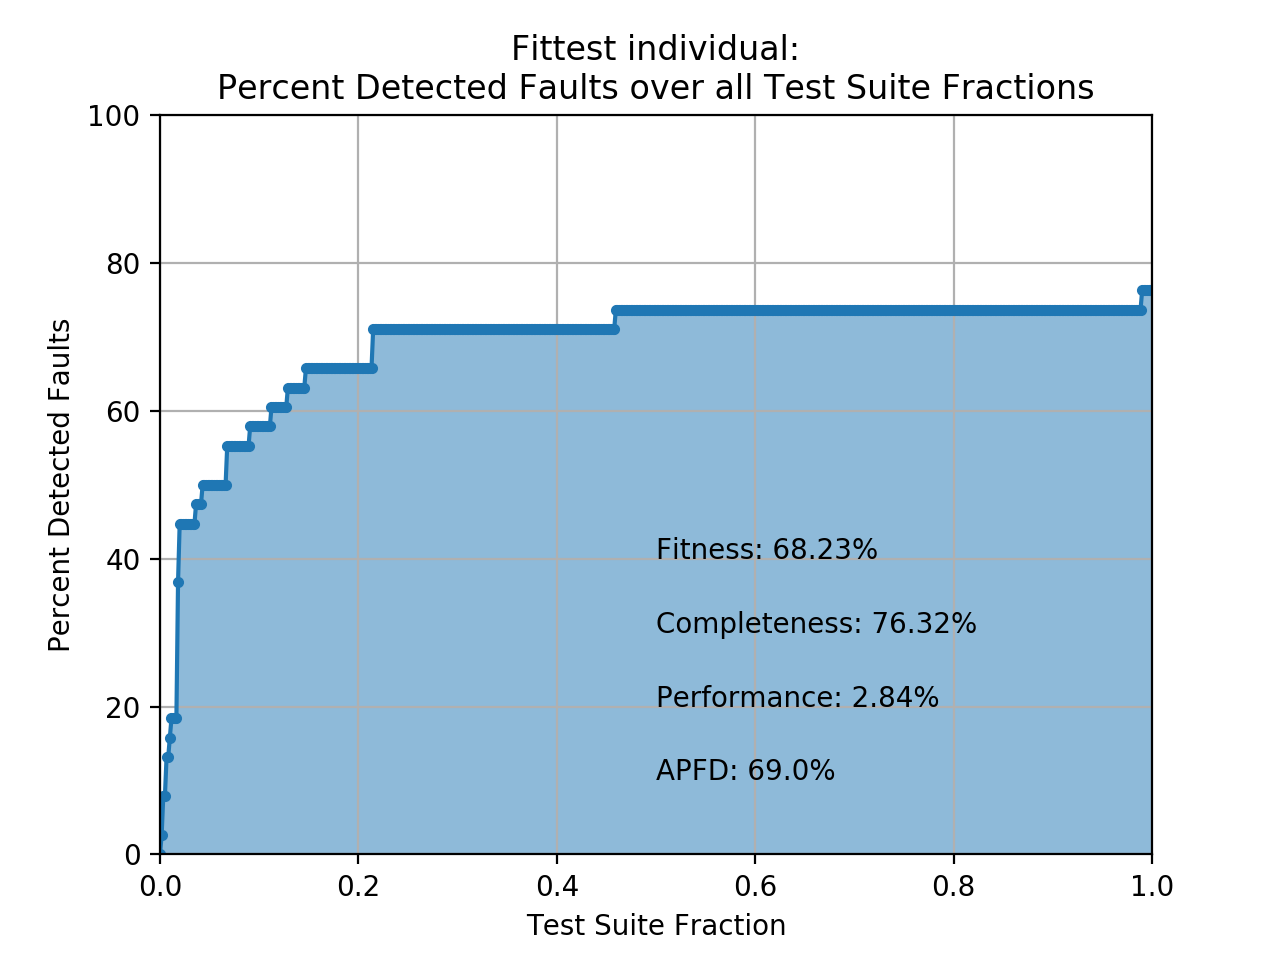
\includegraphics[width=0.49\textwidth]{hill_climber_big_apfd_total}
  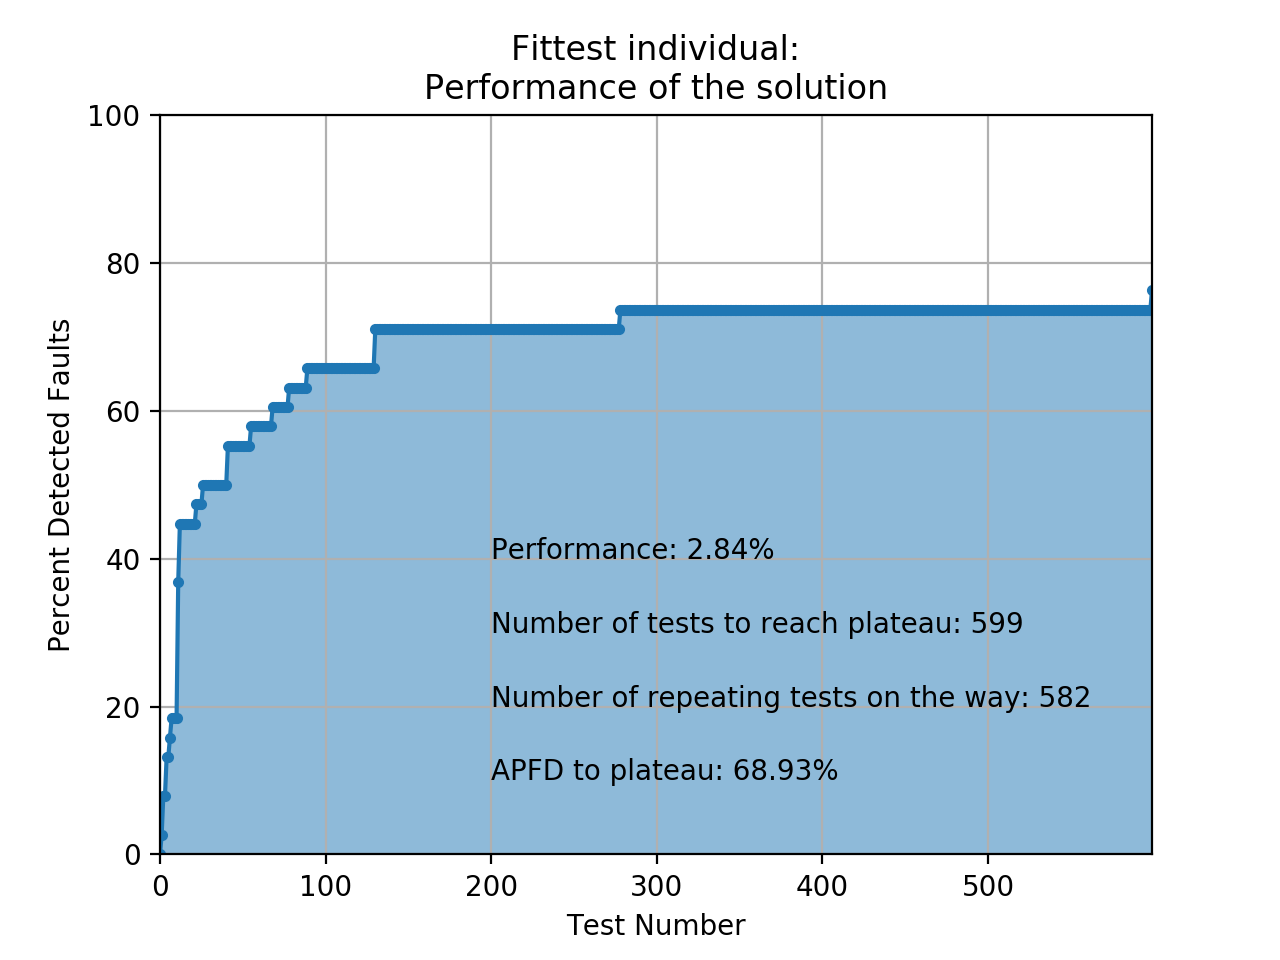
\includegraphics[width=0.49\textwidth]{hill_climber_big_apfd_local}
  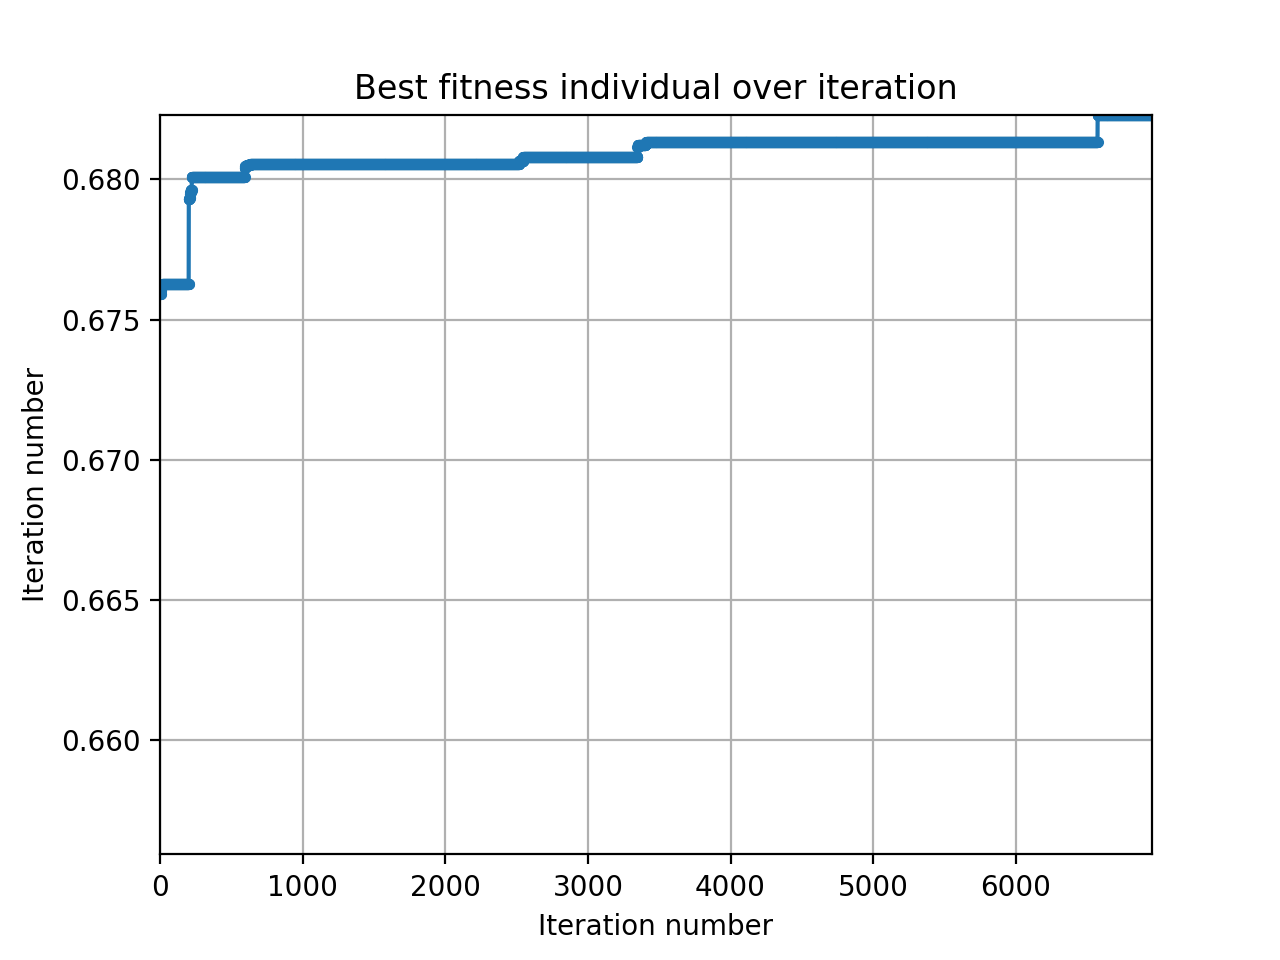
\includegraphics[width=0.6\textwidth]{hill_climber_big_fitness_all}
  \caption{Statistics of running hill climber algorithm over big data set}
  \label{fig:hill_climber_big}
\end{figure}

\begin{figure}[H]
  \centering
  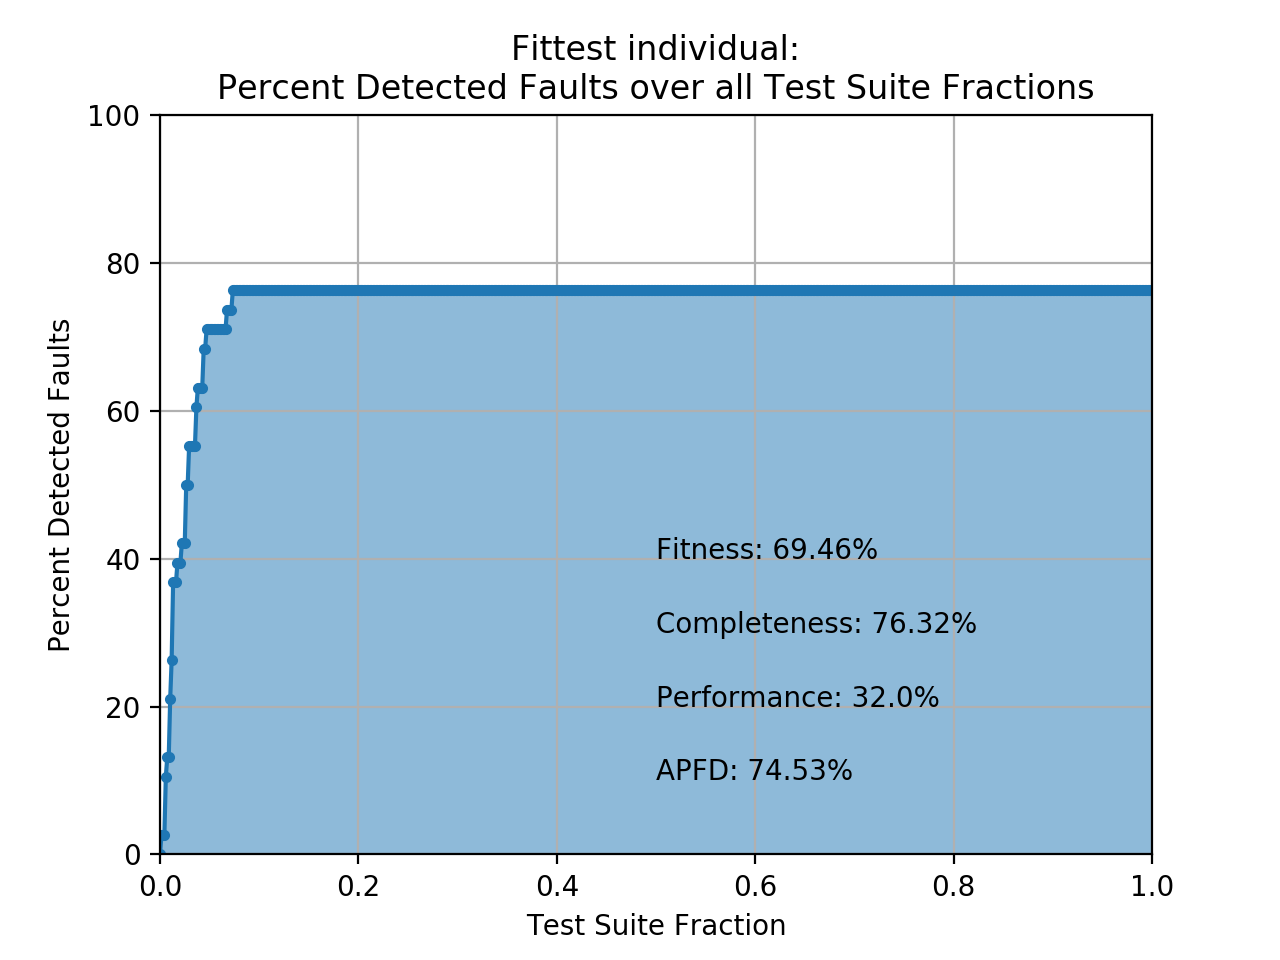
\includegraphics[width=0.49\textwidth]{random_big_apfd_total}
  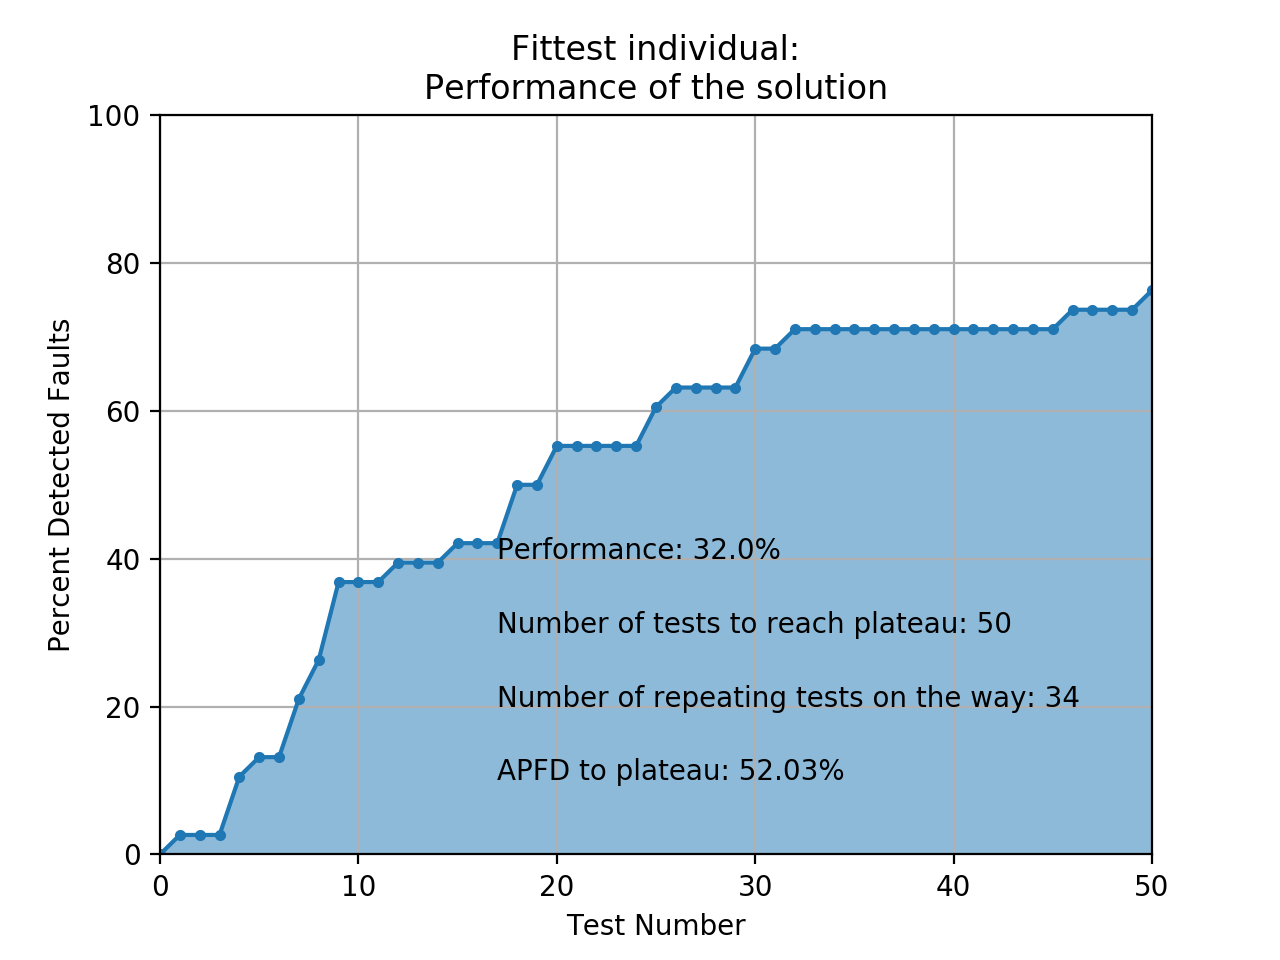
\includegraphics[width=0.49\textwidth]{random_big_apfd_local}
  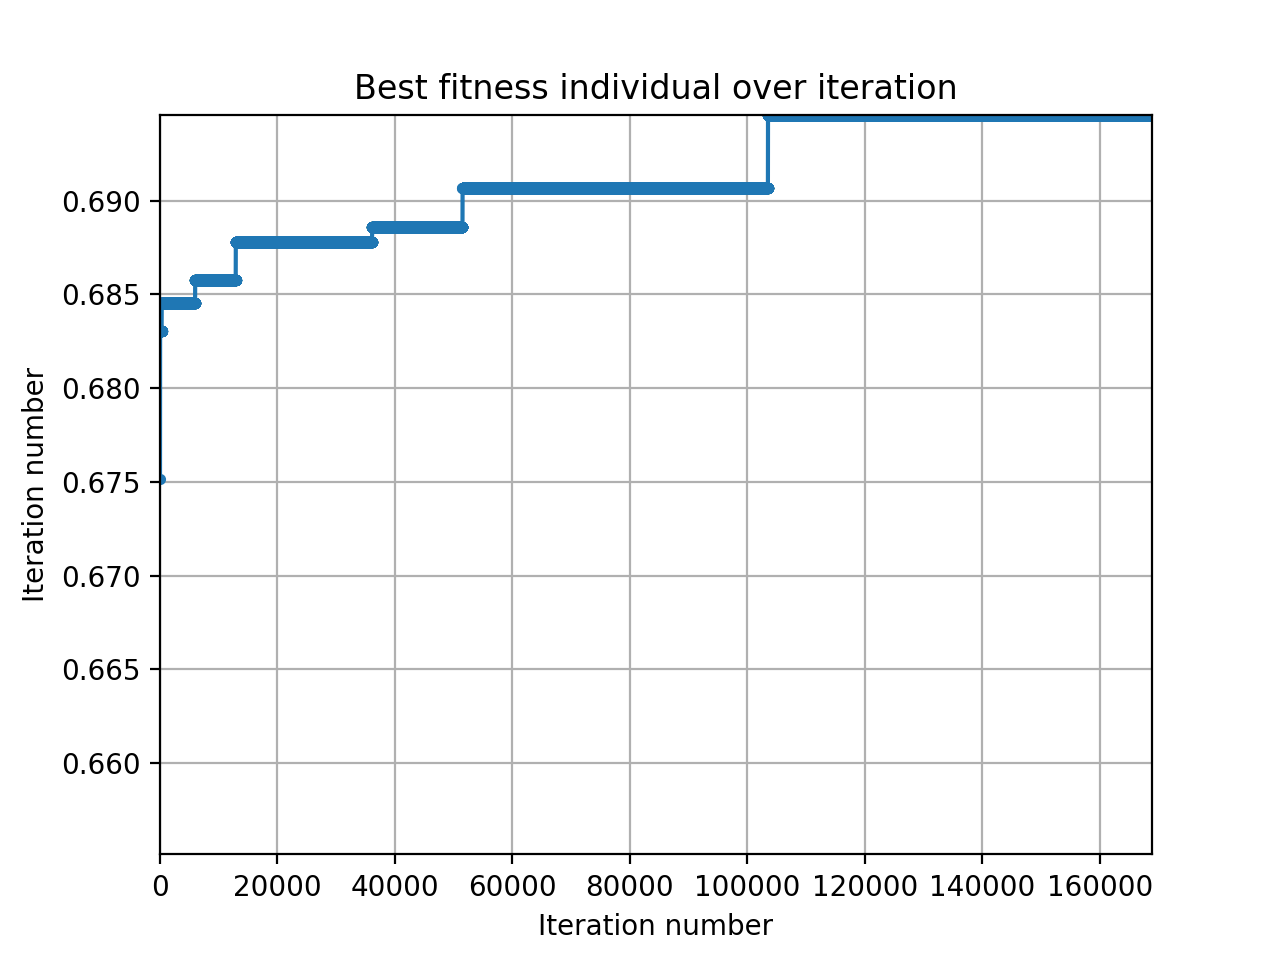
\includegraphics[width=0.6\textwidth]{random_big_fitness_all}
  \caption{Statistics of running random algorithm over big data set}
  \label{fig:random_big}
\end{figure}


Big dataset required much more data crunching and in this scenario, all algorithms again scored the highest possible completeness score of 76.32\% (in this dataset, some faults remained undiscovered, even if all the tests were performed), which proves that at the very least, all algorithms can give the correct solution . However, this time only the genetic algorithm provided most optimal solution with none repeating steps, thus scoring 100\%  performance score and 55.86\% local APFD  compared to 32\% perfomance score  of random algorithm (34 repeating steps to the plateau, 52.03\% local APFD), and a mere 2.84\% performance score, 68.93\% local APFD  of the hill climber (a whopping 582 repeating steps!). Genetic algorithm also had the best total APFD at 75.61\%, compared to 74.53\% random algorithm and 69\% Hill Climber.


\subsection{Conclusion}

With the data fetched from the tests, it can be observed that the genetic algorithm did the best job at finding most optimal solutions to the problem. Second one was the random solver with surprisingly high scores as well. The reason why genetic algorithm solution was better is that while the random solver was just trying to jump across the entire search space to find the solution, the genetic algorithm was making more “educated” guesses while doing it. However, genetic algorithm had a much larger CPU impact, it processed circa 1200 generations of 100 population in 8 minutes for the big dataset, resulting in 120 000 individuals checked. The random algorithm did not have that much CPU impact, hence it could process over 170 000 individuals (see fig 4 and 6 bottom graph). It can be also observed that the genetic algorithm was making a steady progress throughout the execution, while the random algorithm was making a singular jumps in fitness score, by making lucky guesses. The hill climber algorithm meanwhile processed almost 7000 individuals but was scoring much worse results. This is because it was operating in its local search space, trying to improve the initial random solution. The algorithm could be improved by making another candidate a random solution, thus forcing it to check a single random “jump” as in random algorithm. It also yielded much worse performance score, probably because it could not find the best test to add/remove before reaching the plateau - the spikes in the fitness function can be observed on the bottom graph of fig 3 and 5 when it actually succeeded to add/remove/mutate the correct test to improve the score.

\end{document}
